% ============================================================
% Week 2 -- Introduction to linear models (exploratory)
% ============================================================
\chapter{Linear Models: First Look}\label{ch:week02}

This chapter covers Week~2 (Lectures 4--7). The instructor introduces linear models
\emph{exploratorily}, with real and simulated data and R's \texttt{lm}. The formal theory of
estimation starts in \cref{ch:week03}. Week~2 of the official syllabus is ``working with R''.
Here the Python equivalents of every R command are given alongside.

% ============================================================
% Lecture 4 -- Introduction to Linear Models
% ============================================================
\section{Introduction to Linear Models}\label{sec:L04}

\lectureheader{4}{TPJmhTmm4h0}{Week-2 slides \texttt{Feb2.pdf} (recap and ``Model: Aims and Methods'', heights data), with the instructor's handwritten annotations}

\begin{guiding*}
By the end of this lecture you should be able to:
\begin{itemize}
  \item state the aim of modelling: to find a low-dimensional summary of the relationship between a response $y$ and an explanatory variable $x$;
  \item explain ``all models are wrong but some are useful'' with an example;
  \item describe the heights data and use a jittered scatter plot;
  \item explain the training / validation / test split used to judge models.
\end{itemize}
\end{guiding*}

\subsection{Recap}
Week~1 introduced the layered grammar of graphics: scatter plots, smooth lines, bar charts,
polar coordinates and faceting. The instructor calls it the key tool in data visualisation.
Week~2 turns from \emph{looking} at data to \emph{modelling} it. The slides warn that there is
no statistical analysis yet: this week introduces the linear model exploratorily, to see
\emph{how it works}. The formal theory starts in Week~3 (\cref{sec:L08}).

\begin{note}[Practical instruction from the slides]
Download the data sets and the Week-2 R code from the course web page and keep them in the same
directory, set as R's working directory. The Python notebooks follow the same idea. All data
sets are in the project's \texttt{data/} folder, and the notebooks find it by a relative path.
\end{note}

\subsection{Aims of modelling}
\begin{definition}[Response and explanatory variable]\label{def:L04-vars}
We observe pairs $\{(x_i,y_i):1\le i\le n\}$. The variable $x$ is the
\vocab{independent} (explanatory) variable and $y$ the \vocab{dependent} (response)
variable. A \vocab{model} is a low-dimensional summary of the data set that captures the
patterns in the data, and in particular the way $y$ depends on $x$. It can then be used for
\emph{prediction}: given a new $x$, what $y$ should we expect?
\end{definition}

\begin{note}[Caution: all models are wrong, but some are useful]
The slides quote G.\,E.\,P.~Box's aphorism. The instructor's example is the ideal gas law
$PV=RT$. No real gas satisfies it exactly, yet it is a good approximation, and it helps us
\emph{understand the system}. A linear model is judged the same way: not by being true, but by
being a good enough approximation to be useful.
\end{note}

In practice, the slides list the questions one asks:
\begin{itemize}
  \item What hypotheses do we want to test with the data?
  \item How do we judge which model works better? One common method is to split the data into three parts: about $60\%$ for \vocab{training} (fitting the models), $20\%$ for \vocab{query} or validation (choosing between models), and $20\%$ for \vocab{testing} (evaluating the chosen model's performance on data it has never seen).
\end{itemize}

\subsection{The heights data}
\begin{example}[Pearson's mothers and daughters]\label{ex:L04-heights}
Between 1893 and 1898, Karl Pearson (the slides write E.\,S.~Pearson) and his colleagues collected
the heights of mothers and their adult daughters in Britain. The version used in the course
(\texttt{heights.txt}; \texttt{Heights} in the R package \texttt{alr4}) has $n=1375$ pairs. The
annotations mention ``about 1500 odd'' and the restriction to daughters aged at least $18$
and mothers under $65$.
\begin{itemize}
  \item \texttt{Mheight}: height of the mother (inches), mean $62.45$;
  \item \texttt{Dheight}: height of one adult daughter (inches), mean $63.75$.
\end{itemize}
The \emph{object of study} is the question: \emph{how does the daughter's height depend on the
height of the mother?}
\end{example}

Heights were rounded to the nearest inch in the original records, so many points coincide. A
\vocab{jitter plot} moves each data point by a small uniformly distributed amount, here
$U(-0.5,0.5)$ in each coordinate, so that overlapping points become visible.

\begin{figure}[ht]
\centering
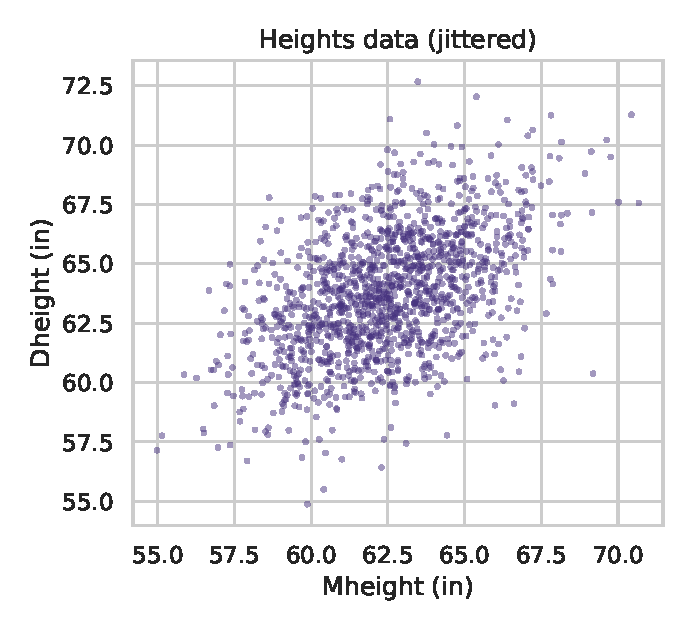
\includegraphics[width=0.5\textwidth]{figures/L04_heights.pdf}
\caption{Jittered scatter plot of daughter's height against mother's height.}
\label{fig:L04-heights}
\end{figure}

The instructor then restricts attention to the middle of the plot: mothers between about $58$
and $68$ inches. His annotations point out two features. There are \emph{no unusually tall
daughters of short mothers}, and \emph{no short daughters of very tall mothers}. The scatter
drifts upwards: taller mothers tend to have taller daughters. The plan is to develop a
technique that fits a linear model to the data $\{(x_i,y_i)\}$, that is, to find $a_1,a_2$ such
that
\[
y = a_1 + a_2 x
\]
is a good approximation. The technique is least squares. It is built step by step in
\cref{sec:L05}. It can also identify outliers: points far from the fitted line.

\begin{note}[Supplementary: the fitted line and ``regression to the mean'']
Anticipating \cref{sec:L05}, the least-squares line for these data is
\[
\widehat{\text{Dheight}} = 29.917 + 0.542\,\text{Mheight}, \qquad R^2 = 0.241.
\]
The slope $0.54<1$ means that a mother who is $1$ inch taller than average has a daughter who is
on average only about half an inch taller than average. This is Galton's \emph{regression to the
mean}. The word ``regression'' comes from this phenomenon. $R^2$ is defined in \cref{sec:L17}.
Only about a quarter of the variation in daughters' heights is explained by mothers' heights.
\end{note}

\begin{figure}[ht]
\centering
\begin{tikzpicture}[>=stealth]
\draw[->] (0,0) -- (7,0) node[right] {$x$};
\draw[->] (0,0) -- (0,4.2) node[above] {$y$};
\foreach \x/\y in {0.8/1.4,1.3/1.1,1.8/2.0,2.4/1.7,3.0/2.6,3.5/2.2,4.1/3.1,4.6/2.8,5.2/3.6,5.8/3.3,6.3/3.9}
  \fill (\x,\y) circle (1.5pt);
\draw[thick,red] (0.4,1.0) -- (6.6,3.9) node[right] {$y=a_1+a_2x$};
\draw[blue,dashed] (3.5,2.2) -- (3.5,2.38);
\draw[blue,dashed] (4.1,3.1) -- (4.1,2.66);
\node[blue,font=\small] at (4.9,1.4) {residual $=y_i-(a_1+a_2x_i)$};
\draw[blue,->] (4.5,1.6) -- (4.12,2.8);
\end{tikzpicture}
\caption{The goal: a line $y=a_1+a_2x$ that summarises the cloud of points. The vertical gaps
are the residuals studied in \cref{sec:L05,sec:L06}.}
\label{fig:L04-line}
\end{figure}

\subsection{Computation}
The R code reads \texttt{heights.txt} and plots \texttt{Dheight} against \texttt{Mheight}, with
jitter. In Python:
\codeline{h = pd.read\_csv(DATA / "Heights.csv"); plt.scatter(h.mheight + rng.uniform(-.5,.5,len(h)), h.dheight + rng.uniform(-.5,.5,len(h)))}
The notebook \nb{week02/L04\_intro\_linear\_models.ipynb} also demonstrates a 60/20/20 split.

\subsection{Summary}
\begin{itemize}
  \item A model is a low-dimensional summary of how the response $y$ depends on $x$. It is used for understanding and prediction.
  \item All models are wrong, but some are useful ($PV=RT$).
  \item Heights data: $1375$ mother--daughter pairs. Jittering reveals overlapping points. Taller mothers tend to have taller daughters.
  \item Goal: find $a_1,a_2$ so that $y\approx a_1+a_2x$. Models are compared using training/validation/test splits.
\end{itemize}

\subsection{Exercises}
\begin{problem}\label{prob:L04-1}
Why does jittering by $U(-0.5,0.5)$ not change any conclusion drawn from the plot, while it would change a fitted line if we fitted to the jittered data? By how much can the mean of the jittered $x$'s differ from the true mean in expectation?
\end{problem}
\begin{problem}\label{prob:L04-2}
Split the heights data at random into $60/20/20$ parts (with a fixed seed). Fit the line to the training part and compute the mean squared prediction error on the test part.
\end{problem}
\begin{problem}\label{prob:L04-3}
Give another physical law (like $PV=RT$) that is ``wrong but useful'', and say in what regime it fails.
\end{problem}
\begin{problem}\label{prob:L04-4}
Suppose daughters' heights were \emph{exactly} equal to their mothers'. What would the scatter plot look like, and what would $a_1,a_2$ be?
\end{problem}

\subsection{Further reading}
Weisberg, \emph{Applied Linear Regression} (4th ed.), Chapter~1 (Scatterplots and Regression),
which is the source of the heights, Forbes, bass and snowfall examples. Wickham \& Grolemund,
\emph{R for Data Science}, ``Model basics''. Christensen, Chapter~6 (Regression analysis) for
the formal treatment.

% ============================================================
% Lecture 5 -- Basics of Linear Models
% ============================================================
\section{Basics of Linear Models}\label{sec:L05}

\lectureheader{5}{Ec94oyf3bKw}{Week-2 slides \texttt{Feb2.pdf} (``Linear Models'' slides on the \texttt{sim1} data), with annotations; Week-2 R code}

\begin{guiding*}
By the end of this lecture you should be able to:
\begin{itemize}
  \item describe a family of linear models $y=a_1+a_2x$ and the residuals of each member;
  \item explain why the \emph{sum of squared} residuals is the criterion used to choose the best line;
  \item find the best line numerically (\texttt{optim}) and with \texttt{lm};
  \item derive the least-squares estimates $\hat a_2=S_{xy}/S_{xx}$, $\hat a_1=\bar y-\hat a_2\bar x$.
\end{itemize}
\end{guiding*}

\subsection{Recap and motivation}
In \cref{sec:L04} we set ourselves the goal of finding $a_1,a_2$ such that $y\approx a_1+a_2x$.
To see how this works, the instructor uses a simulated data set in which we know there is a
linear pattern: \texttt{sim1}, from the R package \texttt{modelr}.

\subsection{A family of lines}
\begin{example}[The \texttt{sim1} data]\label{ex:L05-sim1}
\texttt{sim1} has $n=30$ points: three $y$-values at each of $x=1,2,\dots,10$. The scatter plot
shows a clear pattern: a linear relationship. To explore possible models, the instructor
generates $250$ lines $y=a_1+a_2x$, with the intercept $a_1$ chosen uniformly from $[-20,40]$ and
the slope $a_2$ uniformly from $[-5,5]$, and plots all $250$ lines on top of the data
(\cref{fig:L05-sim1}, left). Most of them are terrible. A few pass through the cloud of points.
\end{example}

To say which lines are good, we need a number that measures how far a line is from the data.
\begin{definition}[Residual]\label{def:L05-residual}
For the model $y=a_1+a_2x$ and the data point $(x_i,y_i)$, the \vocab{residual} is
\[
e_i(a_1,a_2)=y_i-(a_1+a_2x_i),
\]
the vertical distance (with sign) between the data point and the line. It is the part of $y_i$
that the model does not explain.
\end{definition}

The slides then choose one line from the $250$ (line number $130$), plot it, and draw the
residuals as vertical segments from each point to the line. A good line should make the
residuals small \emph{overall}. The instructor's annotation lists candidate criteria:
\begin{enumerate}
  \item minimise the sum of distances $\sum_i \abs{e_i}$ (``hard'', since $\abs{\cdot}$ is not differentiable);
  \item minimise the sum of squared distances $\sum_i e_i^2$: the \vocab{least squares} criterion (ticked on the slide).
\end{enumerate}

\begin{definition}[Least squares line]\label{def:L05-LS}
For data $\{(x_i,y_i)\}_{i=1}^n$ let
\[
f(a_1,a_2)=\sum_{i=1}^n \bigl(y_i-a_1-a_2x_i\bigr)^2 .
\]
A pair $(\hat a_1,\hat a_2)$ minimising $f$ gives the \vocab{least squares line}
$y=\hat a_1+\hat a_2 x$.
\end{definition}

\subsection{Finding the best line numerically}
The R code on the slides defines the model and a distance, then minimises the distance with a
general-purpose optimiser:
\begin{center}
\begin{minipage}{0.8\textwidth}\small\ttfamily
model1 <- function(a, data) \{ a[1] + data\$x * a[2] \}\\
measure\_distance <- function(mod, data) \{\\
\quad diff <- data\$y - model1(mod, data)\\
\quad sqrt(mean(diff\textasciicircum 2)) \}\\
best <- optim(c(0, 0), measure\_distance, data = sim1)\\
best\$par \qquad\qquad \# 4.222248 2.051204\\
measure\_distance(best\$par, sim1) \# 2.128181
\end{minipage}
\end{center}
The distance used is the \vocab{root mean squared error}
$\mathrm{RMSE}(a_1,a_2)=\sqrt{\tfrac1n\sum_i e_i(a_1,a_2)^2}=\sqrt{f(a_1,a_2)/n}$. The map
$t\mapsto\sqrt{t/n}$ is strictly increasing, so minimising RMSE is the same as minimising $f$.
\texttt{optim} (Nelder--Mead) returns intercept $4.222248$ and slope $2.051204$, with
RMSE $2.128181$. The slide plots this line: intercept $\approx 4.22$, slope $\approx 2.05$. It
seems to give a good approximation.

The slide then asks: \emph{how do we judge the model, and is this the best possible solution?}
The ``to do'' written on the slide is to minimise $f(a_1,a_2)$ exactly. R's built-in function
\texttt{lm(y \textasciitilde\ x, data = sim1)} does this and returns
\[
\hat a_1 = 4.220822,\qquad \hat a_2=2.051533 .
\]
The small difference from \texttt{optim} is numerical: Nelder--Mead stops once further progress
falls below its tolerance. \texttt{lm} solves the problem exactly, as we now show.

\subsection{The least-squares estimates}
\begin{theorem}[Least squares for a straight line]\label{thm:L05-slr}
Let $n\ge 2$ and suppose the $x_i$ are not all equal. Write
\[
\bar x=\tfrac1n\sum x_i,\quad \bar y=\tfrac1n\sum y_i,\quad
S_{xx}=\sum_{i}(x_i-\bar x)^2,\quad S_{xy}=\sum_i (x_i-\bar x)(y_i-\bar y).
\]
Then $f(a_1,a_2)=\sum(y_i-a_1-a_2x_i)^2$ has a unique minimiser
\[
\hat a_2=\frac{S_{xy}}{S_{xx}},\qquad \hat a_1=\bar y-\hat a_2\,\bar x ,
\]
and the minimum value is $f(\hat a_1,\hat a_2)=S_{yy}-S_{xy}^2/S_{xx}$, where $S_{yy}=\sum(y_i-\bar y)^2$.
\end{theorem}
\begin{proof}
We complete the square twice, so that no calculus is needed. For fixed $a_2$ write
$z_i=y_i-a_2x_i$. Then $f=\sum_i(z_i-a_1)^2$. By \cref{prop:L01-bestconst},
\[
\sum_i (z_i-a_1)^2=\sum_i (z_i-\bar z)^2+n(\bar z-a_1)^2,\qquad \bar z=\bar y-a_2\bar x .
\]
Now $z_i-\bar z=(y_i-\bar y)-a_2(x_i-\bar x)$, so
\[
\sum_i (z_i-\bar z)^2=S_{yy}-2a_2S_{xy}+a_2^2S_{xx}
= S_{xx}\Bigl(a_2-\frac{S_{xy}}{S_{xx}}\Bigr)^2 + S_{yy}-\frac{S_{xy}^2}{S_{xx}} ,
\]
where we used $S_{xx}>0$ (the $x_i$ are not all equal). Altogether
\[
f(a_1,a_2)= S_{yy}-\frac{S_{xy}^2}{S_{xx}} + S_{xx}\Bigl(a_2-\frac{S_{xy}}{S_{xx}}\Bigr)^2 + n\bigl(\bar y-a_2\bar x-a_1\bigr)^2 .
\]
The last two terms are non-negative. Both vanish if and only if $a_2=S_{xy}/S_{xx}$ and
$a_1=\bar y-a_2\bar x$. Hence this pair is the unique minimiser, and the minimum is
$S_{yy}-S_{xy}^2/S_{xx}$.
\end{proof}

\begin{corollary}\label{cor:L05-props}
The least-squares line passes through $(\bar x,\bar y)$. The residuals
$\hat e_i=y_i-\hat a_1-\hat a_2x_i$ satisfy $\sum_i\hat e_i=0$ and $\sum_i x_i\hat e_i=0$.
\end{corollary}
\begin{proof}
At $x=\bar x$ the line gives $\hat a_1+\hat a_2\bar x=\bar y$. Next,
$\hat e_i=(y_i-\bar y)-\hat a_2(x_i-\bar x)$. Summing gives $0-0=0$. Also
$\sum_i (x_i-\bar x)\hat e_i=S_{xy}-\hat a_2S_{xx}=0$. Since $\sum\hat e_i=0$, it follows that
$\sum x_i\hat e_i=\sum(x_i-\bar x)\hat e_i+\bar x\sum\hat e_i=0$.
\end{proof}
The two identities $\sum\hat e_i=0$ and $\sum x_i\hat e_i=0$ are exactly the \emph{normal
equations} of \cref{sec:L12}, written out for a straight line.

\begin{example}[A least-squares line by hand]\label{ex:L05-hand}
Take $n=4$ points with $x=(1,2,3,4)$ and $y=(2,3,5,6)$.
\begin{itemize}
  \item $\bar x=2.5$ and $\bar y=16/4=4$.
  \item Deviations: $x_i-\bar x=(-1.5,-0.5,0.5,1.5)$ and $y_i-\bar y=(-2,-1,1,2)$.
  \item $S_{xx}=2.25+0.25+0.25+2.25=5$ and $S_{xy}=3+0.5+0.5+3=7$. Also $S_{yy}=4+1+1+4=10$.
  \item $\hat a_2=7/5=1.4$ and $\hat a_1=4-1.4\times 2.5=0.5$.
  \item Fitted values: $0.5+1.4x=(1.9,3.3,4.7,6.1)$. Residuals: $(0.1,-0.3,0.3,-0.1)$. They sum to $0$, and $\sum x_i\hat e_i=0.1-0.6+0.9-0.4=0$.
  \item Minimum: $f=0.01+0.09+0.09+0.01=0.2$, which agrees with $S_{yy}-S_{xy}^2/S_{xx}=10-49/5=0.2$. The RMSE is $\sqrt{0.2/4}=0.2236$.
\end{itemize}
\end{example}

\begin{figure}[ht]
\centering
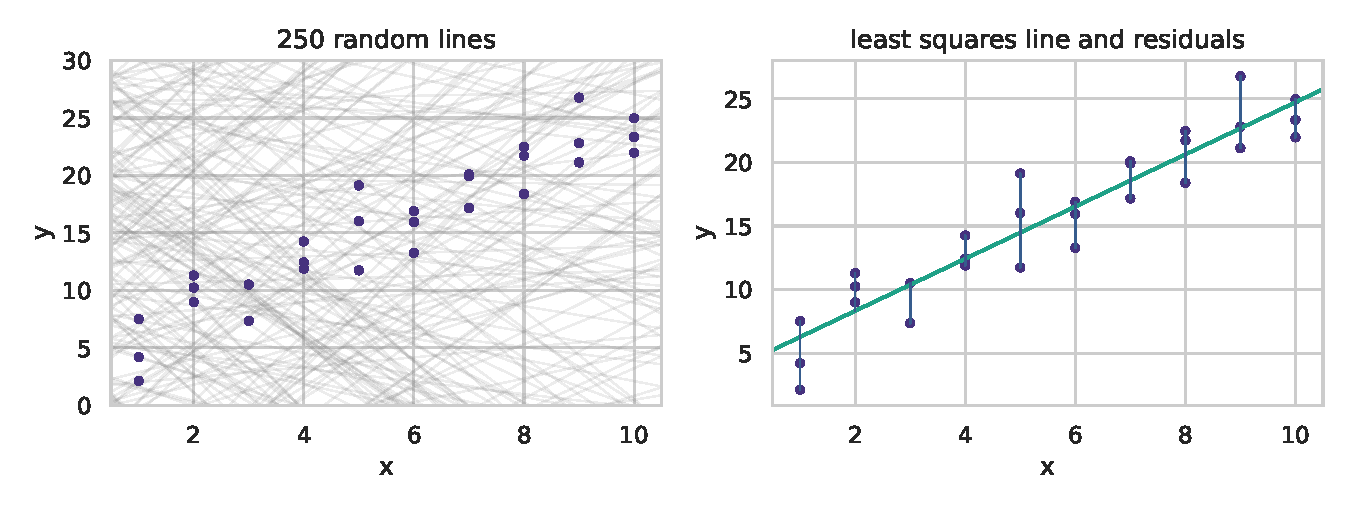
\includegraphics[width=0.95\textwidth]{figures/L05_sim1.pdf}
\caption{Left: $250$ random lines over the \texttt{sim1} data. Right: the least-squares line and its residuals.}
\label{fig:L05-sim1}
\end{figure}

\begin{note}[Supplementary: why squares?]
Squares make $f$ a smooth, convex quadratic, so the minimiser has the closed form of
\cref{thm:L05-slr}. The absolute-value criterion has no closed form and may have many
minimisers. Squares also lead to the Pythagorean geometry of \cref{sec:L12,sec:L14}. Under
normal errors, least squares coincides with maximum likelihood, and the Gauss--Markov theorem
(Week~6) shows that it is optimal among linear unbiased estimators. The price is sensitivity to
outliers: one large residual counts quadratically.
\end{note}

\subsection{Computation}
\begin{center}\small
\begin{tabular}{@{}>{\raggedright\arraybackslash}p{7cm}>{\raggedright\arraybackslash}p{8.4cm}@{}}\hline
R & Python\\\hline
\texttt{runif(250,-20,40)}, \texttt{runif(250,-5,5)} & \texttt{rng.uniform(-20, 40, 250)}, \texttt{rng.uniform(-5, 5, 250)}\\
\texttt{optim(c(0,0), measure\_distance, data=sim1)} & \texttt{scipy.optimize.minimize(rmse, [0,0], method="Nelder-Mead")}\\
\texttt{lm(y \textasciitilde\ x, data=sim1)} & \texttt{smf.ols("y \textasciitilde\ x", data=sim1).fit().params}\\\hline
\end{tabular}
\end{center}
The notebook \nb{week02/L05\_basics\_linear\_models.ipynb} also computes $\hat a_1,\hat a_2$ from
the formulas of \cref{thm:L05-slr} and checks them against \texttt{statsmodels}.

\subsection{Summary}
\begin{itemize}
  \item Residual $e_i=y_i-(a_1+a_2x_i)$. Criterion: minimise $f(a_1,a_2)=\sum e_i^2$ (least squares). This is equivalent to minimising RMSE.
  \item $\hat a_2=S_{xy}/S_{xx}$, $\hat a_1=\bar y-\hat a_2\bar x$, and $\min f=S_{yy}-S_{xy}^2/S_{xx}$.
  \item The fitted line passes through $(\bar x,\bar y)$, and $\sum\hat e_i=\sum x_i\hat e_i=0$.
  \item \texttt{sim1}: \texttt{lm} gives $4.220822$ and $2.051533$ (RMSE $2.128181$). \texttt{optim} agrees to about three decimals.
\end{itemize}

\subsection{Exercises}
\begin{problem}\label{prob:L05-1}
Show that $S_{xy}=\sum_i (x_i-\bar x)y_i=\sum_i x_iy_i-n\bar x\bar y$.
\end{problem}
\begin{problem}\label{prob:L05-2}
Fit the least-squares line by hand to $x=(0,1,2)$, $y=(1,1,4)$. Give the residuals and the minimum of $f$.
\end{problem}
\begin{problem}\label{prob:L05-3}
Show that if we fit the line through the origin, $y=a_2x$, the least-squares slope is $\sum x_iy_i/\sum x_i^2$.
\end{problem}
\begin{problem}\label{prob:L05-4}
What happens in \cref{thm:L05-slr} if all $x_i$ are equal? Describe the set of minimisers.
\end{problem}
\begin{problem}\label{prob:L05-5}
Minimise $\sum\abs{e_i}$ for \texttt{sim1} numerically (Nelder--Mead) and compare the line with the least-squares line.
\end{problem}

\subsection{Further reading}
Wickham \& Grolemund, \emph{R for Data Science}, ``Model basics'' (the \texttt{sim1} example).
Weisberg, \emph{ALR}, Chapter~2 (Simple linear regression). Christensen, Chapter~6.
Rao, \S4a (least squares).

% ============================================================
% Lecture 6 -- More on Linear Models - Residuals
% ============================================================
\section{More on Linear Models: Residuals}\label{sec:L06}

\lectureheader{6}{YlAdFp_3j1M}{Week-2 slides \texttt{Feb2.pdf} (``Linear Models: best line'', Forbes data, residual plots), with annotations; Week-2 R code}

\begin{guiding*}
By the end of this lecture you should be able to:
\begin{itemize}
  \item fit a least-squares line with \texttt{lm} and read off its coefficients;
  \item draw and interpret a \emph{residual plot}: residuals against the explanatory variable;
  \item recognise curvature and outliers from a residual plot;
  \item explain why a transformation (here $\log$) can make a relationship linear.
\end{itemize}
\end{guiding*}

\subsection{Recap}
In \cref{sec:L05} we defined residuals $e_i=y_i-(a_1+a_2x_i)$ and chose the line minimising
$\sum e_i^2$. For \texttt{sim1}, \texttt{lm} returned $(4.220822,\,2.051533)$. This lecture
applies the method to real data. It also shows that the residuals left over after fitting are
the main diagnostic tool: they tell us whether a straight line was the right model in the first
place.

\subsection{Forbes' boiling-point data}
\begin{example}[Forbes, 1857]\label{ex:L06-forbes}
In the 1840s and 1850s the Scottish physicist James D.~Forbes collected data in the Alps and in
Scotland. He wanted to estimate altitude from the \emph{boiling point of water}, which could
replace the fragile barometers of the time. The data set (\texttt{forbes.txt}; \texttt{Forbes}
in \texttt{alr4}) has $n=17$ pairs:
\begin{itemize}
  \item \texttt{bp} = boiling point of water ($^\circ$F), from $194.3$ to $212.2$;
  \item \texttt{pres} = atmospheric pressure (inches of mercury), from $20.79$ to $30.06$.
\end{itemize}
The slides plot \texttt{Pressure} against \texttt{Temperature} and use \texttt{lm} to find the
best line.
\end{example}

Fitting $\text{pres} = a_1 + a_2\,\text{bp}$ by least squares gives
\[
\widehat{\text{pres}}=-81.0637+0.5229\,\text{bp}.
\]
In the scatter plot the points lie very close to this line, and $R^2=0.9944$. Judged by the
scatter plot alone, the fit looks almost perfect.

\begin{definition}[Residual plot]\label{def:L06-residplot}
For a fitted line $\hat y_i=\hat a_1+\hat a_2x_i$, the \vocab{fitted residuals} are
$\hat e_i=y_i-\hat y_i$. A \vocab{residual plot} plots $\hat e_i$ against $x_i$ (or against
$\hat y_i$). If the straight-line model is adequate, the residual plot should look like a
structureless horizontal band around $0$.
\end{definition}

The residual plot for Forbes' data (\cref{fig:L06-forbes}, bottom left) tells a different story.
The instructor's annotations mark:
\begin{itemize}
  \item the \emph{largest positive residual}: case $12$ ($\text{bp}=204.6$), with $\hat e_{12}=0.650$, far above all the others;
  \item the \emph{most negative} residual: case $11$ ($\text{bp}=203.6$), with $\hat e_{11}=-0.257$;
  \item a \emph{curved} pattern in the rest. The residuals are positive at both ends (e.g.\ $0.151, 0.256$ at the lowest temperatures and $0.143, 0.166$ at the highest) and negative in the middle.
\end{itemize}
A systematic curve in the residuals means that the straight line is not the right shape. It
underestimates at the ends and overestimates in the middle. The residual plot magnifies
departures from the line that the scatter plot hides, because it removes the large linear trend.

\begin{figure}[ht]
\centering
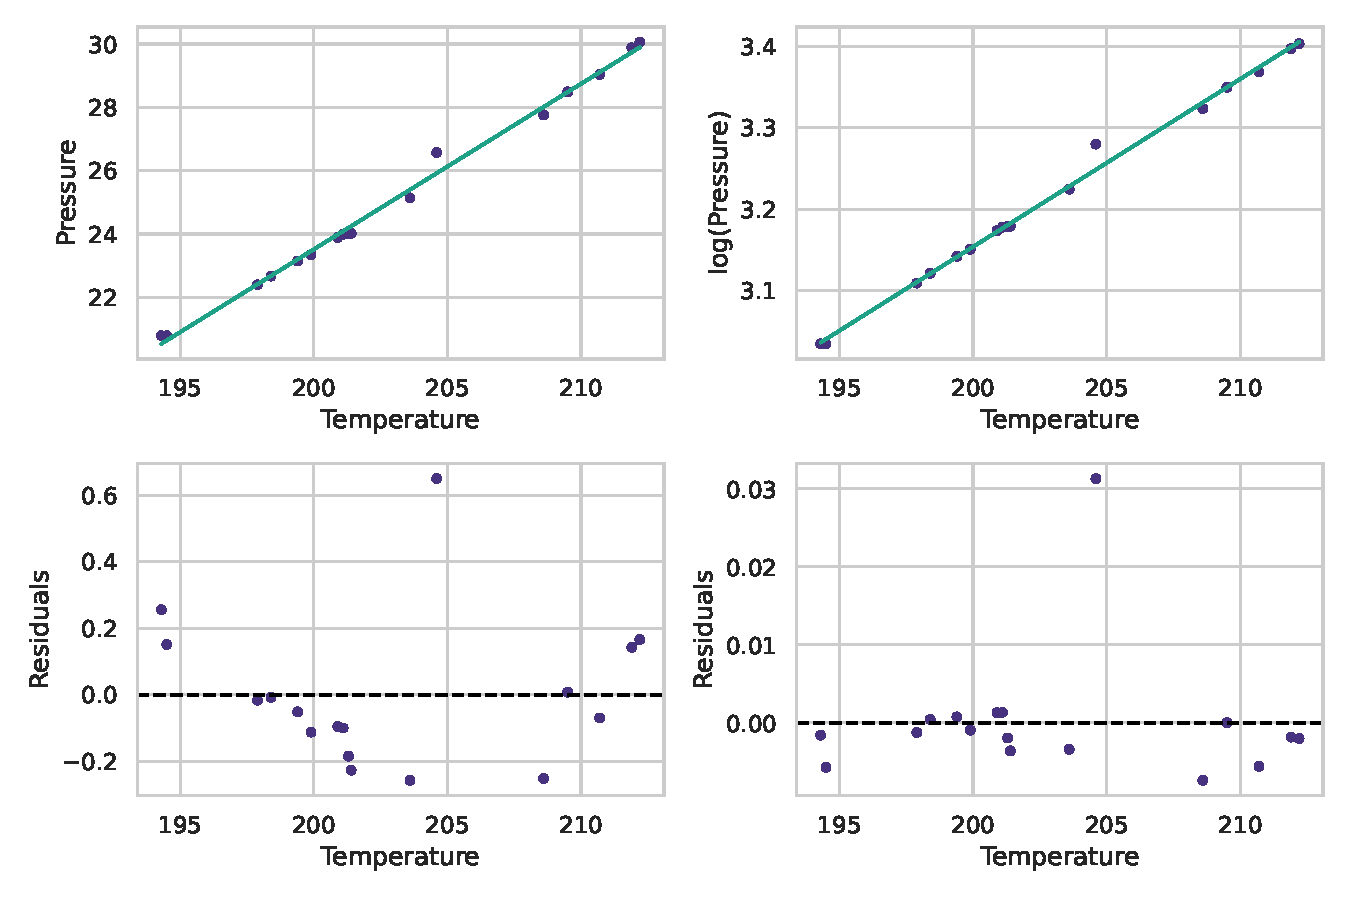
\includegraphics[width=0.9\textwidth]{figures/L06_forbes.pdf}
\caption{Forbes' data. Top: fitted lines for Pressure and for $\log$(Pressure). Bottom: the
corresponding residual plots. Curvature is visible on the left; on the right only case 12 stands out.}
\label{fig:L06-forbes}
\end{figure}

\subsection{A transformation}
The slides then note that \emph{physical theory} says that $\log(\text{Pressure})$ is linearly
related to temperature. We therefore fit
\[
\log(\text{pres}) = a_1 + a_2\,\text{bp}.
\]
With natural logarithms, least squares gives
$\widehat{\log(\text{pres})}=-0.97087+0.020622\,\text{bp}$. The \texttt{alr4} file also contains
\texttt{lpres} $=100\log_{10}(\text{pres})$, which gives $-42.138+0.8955\,\text{bp}$. The two fits
are equivalent up to the constant factor $100/\ln 10$. The residual plot (bottom right) no longer
shows curvature: apart from case~12, the residuals form a horizontal band. Case~12, with residual
$0.0313$ on the log scale, is now clearly an \emph{outlier}. It could be a recording error.

\begin{note}[Supplementary: the physics behind the log]
The Clausius--Clapeyron relation says that the vapour pressure $P$ of a liquid at absolute
temperature $T$ satisfies, approximately, $\log P = c - L/(RT)$. Here $L$ is the latent heat
and $R$ is the gas constant. Water boils when its vapour pressure equals the atmospheric
pressure, so $\log(\text{pres})$ is linear in $1/T$. Over the narrow range
$194$--$212\,^\circ$F (about $363$--$373$\,K), $1/T$ is itself very nearly linear in $T$. This is
why $\log(\text{pres})$ is linear in bp to high accuracy.
\end{note}

\begin{note}[Supplementary: what one outlier does]
Refitting the log model without case~12 gives $\widehat{\log(\text{pres})}=-0.95177+0.020519\,\text{bp}$,
and $R^2$ rises from $0.99496$ to $0.99957$. The slope hardly changes, so the outlier does not
distort the line much. Its main effect is to inflate the residual variance. Whether to delete an
outlier is a scientific decision, not a statistical one. It should be reported either way.
\end{note}

\begin{proposition}[Supplementary: residuals carry no linear trend]\label{prop:L06-noline}
If a least-squares line is fitted to $(x_i,y_i)$, then the least-squares line fitted to the
residual plot $(x_i,\hat e_i)$ is the horizontal line $y=0$.
\end{proposition}
\begin{proof}
By \cref{thm:L05-slr}, the slope for the data $(x_i,\hat e_i)$ is
$\sum_i (x_i-\bar x)(\hat e_i-\bar{\hat e})/S_{xx}$. By \cref{cor:L05-props},
$\bar{\hat e}=0$ and $\sum_i (x_i-\bar x)\hat e_i=0$, so the slope is $0$. The intercept is then
$\bar{\hat e}-0\cdot\bar x=0$.
\end{proof}
So any \emph{linear} tendency is removed by the fit. What remains visible in a residual plot is
non-linear structure (curvature), unequal spread, or unusual points. These are exactly the
features we look for.

\subsection{Computation}
\begin{center}\small
\begin{tabular}{@{}>{\raggedright\arraybackslash}p{7cm}>{\raggedright\arraybackslash}p{8.4cm}@{}}\hline
R & Python\\\hline
\texttt{m <- lm(pres \textasciitilde\ bp, data = forbes)} & \texttt{m = smf.ols("pres \textasciitilde\ bp", data=fb).fit()}\\
\texttt{residuals(m)} & \texttt{m.resid}\\
\texttt{plot(forbes\$bp, residuals(m))} & \texttt{plt.scatter(fb.bp, m.resid)}\\
\texttt{lm(log(pres) \textasciitilde\ bp, data = forbes)} & \texttt{smf.ols("np.log(pres) \textasciitilde\ bp", data=fb).fit()}\\\hline
\end{tabular}
\end{center}
See \nb{week02/L06\_residuals.ipynb}.

\subsection{Summary}
\begin{itemize}
  \item Residual plot: $\hat e_i$ against $x_i$. It should be a structureless band around $0$.
  \item Forbes: $\widehat{\text{pres}}=-81.06+0.523\,\text{bp}$. The residuals are curved, case 12 has the largest positive residual ($0.650$) and case 11 the most negative ($-0.257$).
  \item $\log(\text{pres})$ is linear in bp (physical theory). After transforming, only the outlier (case 12) remains.
  \item The fitted residuals have zero mean and zero correlation with $x$, so only non-linear structure can show up.
\end{itemize}

\subsection{Exercises}
\begin{problem}\label{prob:L06-1}
Show that $\sum_i \hat y_i\hat e_i=0$ for a least-squares line. Deduce that plotting residuals against fitted values also shows no linear trend.
\end{problem}
\begin{problem}\label{prob:L06-2}
Refit Forbes' log model without case $12$ in Python and confirm the coefficients $-0.95177$ and $0.020519$.
\end{problem}
\begin{problem}\label{prob:L06-3}
Show that if $\text{lpres}=100\log_{10}(\text{pres})$, the least-squares coefficients for lpres are exactly $100/\ln 10$ times those for $\ln(\text{pres})$.
\end{problem}
\begin{problem}\label{prob:L06-4}
Describe the residual plot you would expect if the spread of $y$ around the true line grew with $x$.
\end{problem}

\subsection{Further reading}
Weisberg, \emph{ALR}, Chapter~1 (Forbes' data) and Chapter~9 (outliers and diagnostics).
Christensen, Chapter~12 (Model diagnostics).

% ============================================================
% Lecture 7 -- Play with more data sets in R
% ============================================================
\section{Playing with More Data Sets}\label{sec:L07}

\lectureheader{7}{V8SQrXbSA44}{Week-2 slides \texttt{Feb2.pdf} (smallmouth bass and snowfall examples), with annotations; Week-2 data sets \texttt{wblake.txt}, \texttt{snow.txt}}

\begin{guiding*}
By the end of this lecture you should be able to:
\begin{itemize}
  \item explore a data set with a discrete explanatory variable (age) and compare the mean response at each level with a fitted line;
  \item explain why a regression of $y$ on $x$ cannot simply be inverted to predict $x$ from $y$;
  \item recognise from a scatter plot and a fitted line when two variables are essentially unrelated.
\end{itemize}
\end{guiding*}

\subsection{Recap}
We can fit a least-squares line (\cref{sec:L05}) and check it with a residual plot
(\cref{sec:L06}). The instructor now applies the same steps to further data sets from
Weisberg's book. The point is to see how scatter plots guide the choice of a model.

\subsection{Length at age for smallmouth bass}
\begin{example}[West Bearskin Lake bass]\label{ex:L07-bass}
The data (\texttt{wblake.txt}; \texttt{wblake} in \texttt{alr4}) record the \texttt{Length}
(mm) and \texttt{Age} (years) of $n=439$ smallmouth bass caught in West Bearskin Lake, Minnesota,
USA, in 1991. Age is determined from annular rings on the fish's scales, like the rings of a
tree. Ages run from $1$ to $8$, with counts
\begin{center}
\begin{tabular}{lcccccccc}\hline
Age & 1 & 2 & 3 & 4 & 5 & 6 & 7 & 8\\
number of fish & 38 & 72 & 94 & 15 & 68 & 87 & 61 & 4\\\hline
\end{tabular}
\end{center}
\end{example}

Because Age is discrete, the scatter plot consists of eight vertical strips. Within each strip
there is a spread of lengths. Fish of the same age differ in length. We can summarise each strip
by its mean length and compare the eight means with the least-squares line
\[
\widehat{\text{Length}} = 65.53 + 30.32\,\text{Age}.
\]
The means lie close to the line for young fish but bend below it for the oldest: growth slows
with age. The instructor's annotation makes a second point. The graph shows how length
depends on age, but \emph{we cannot use the line to predict age from length}. Each strip is wide,
and the strips overlap heavily. A fish of length $200$\,mm could plausibly be $3$, $4$ or $5$
years old. Moreover, inverting the line $y=a_1+a_2x$ is not the same as regressing $x$ on $y$.

\begin{proposition}[Supplementary: regression is not symmetric]\label{prop:L07-asym}
Let $\hat a_2^{(y|x)}=S_{xy}/S_{xx}$ be the least-squares slope of $y$ on $x$ and
$\hat b_2^{(x|y)}=S_{xy}/S_{yy}$ the slope of $x$ on $y$. Then
\[
\hat a_2^{(y|x)}\cdot \hat b_2^{(x|y)}=r^2,\qquad r=\frac{S_{xy}}{\sqrt{S_{xx}S_{yy}}} .
\]
The line of $y$ on $x$, rewritten as a line for $x$ in terms of $y$, has slope $1/\hat a_2^{(y|x)}$.
This equals $\hat b_2^{(x|y)}$ only when $r^2=1$, i.e.\ when all points lie exactly on a line.
\end{proposition}
\begin{proof}
Both formulas come from \cref{thm:L05-slr}, with the roles of $x$ and $y$ swapped for the second.
Multiplying, $\hat a_2\hat b_2 = S_{xy}^2/(S_{xx}S_{yy})=r^2$. The equality
$1/\hat a_2=\hat b_2$ is equivalent to $\hat a_2\hat b_2=1$, i.e.\ to $r^2=1$. By the
Cauchy--Schwarz inequality $r^2\le 1$, with equality if and only if the vectors
$(y_i-\bar y)$ and $(x_i-\bar x)$ are proportional.
\end{proof}

\subsection{Predicting the weather: snowfall}
\begin{example}[Fort Collins snowfall]\label{ex:L07-snow}
Can the snowfall of early winter predict the snowfall of late winter? The data (\texttt{snow.txt};
\texttt{ftcollinssnow} in \texttt{alr4}) give, for $93$ years starting in 1900 at Fort Collins,
Colorado, the snowfall (inches) from September to December (\texttt{Early}) and from January to
June (\texttt{Late}).
\end{example}
The scatter plot of Late against Early is a shapeless cloud. The least-squares line is
\[
\widehat{\text{Late}} = 28.64 + 0.2035\,\text{Early},
\]
with $R^2=0.0258$ and sample correlation $r=0.161$. The slope is small and, as we will be able to
test in \cref{sec:L16}, not significantly different from $0$ (p-value $0.124$). The fitted line
is hardly distinguishable from the horizontal line at the mean of Late. The instructor's
conclusion, written on the slide: early and late snowfall are \emph{not related}.
A good-looking line can always be computed. Whether it means anything is a separate question.

\begin{figure}[ht]
\centering
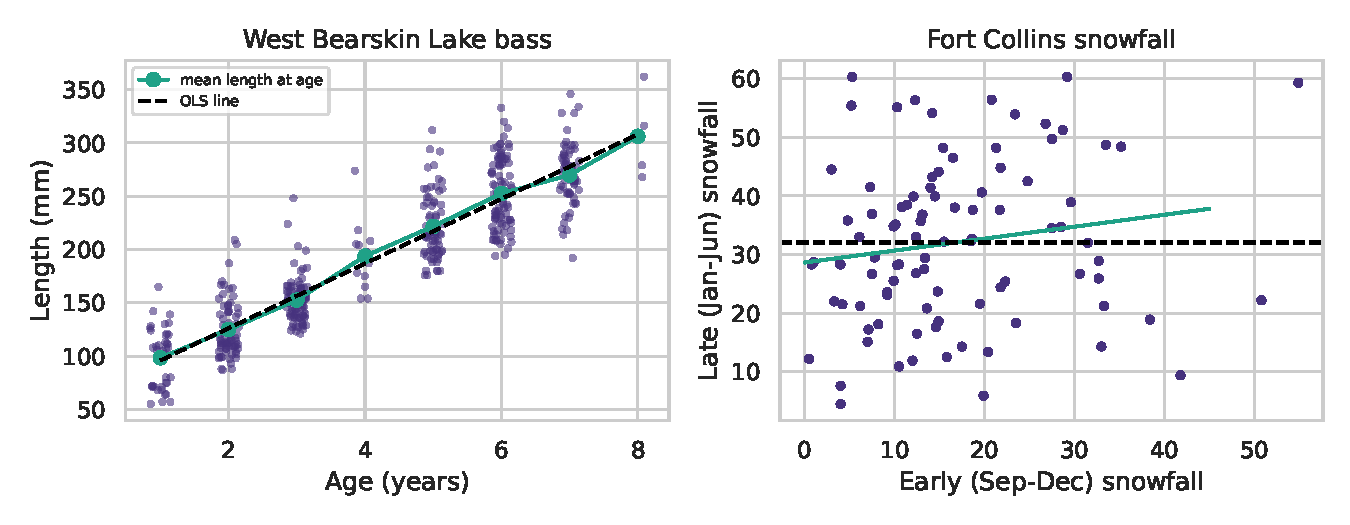
\includegraphics[width=0.95\textwidth]{figures/L07_bass_snow.pdf}
\caption{Left: bass length against age, with mean length at each age and the least-squares line.
Right: late against early snowfall; the fitted line (solid) is close to the mean of Late (dashed).}
\label{fig:L07-bass-snow}
\end{figure}

\subsection{Computation}
The Week-2 R code reads each \texttt{.txt} file, plots it and calls \texttt{lm}. In Python:
\codeline{w = pd.read\_csv(DATA / "wblake.csv"); w.groupby("Age").Length.mean(); smf.ols("Length \textasciitilde\ Age", w).fit()}
\codeline{sn = pd.read\_csv(DATA / "ftcollinssnow.csv"); smf.ols("Late \textasciitilde\ Early", sn).fit().summary()}
See \nb{week02/L07\_more\_datasets.ipynb}.

\subsection{Summary}
\begin{itemize}
  \item Bass: $\widehat{\text{Length}}=65.53+30.32\,\text{Age}$. Mean length grows with age but levels off. Age cannot be predicted reliably from length.
  \item The regressions of $y$ on $x$ and of $x$ on $y$ differ unless $r^2=1$. Their slopes multiply to $r^2$.
  \item Snowfall: slope $0.2035$, $R^2=0.026$. Early and late snowfall are essentially unrelated.
\end{itemize}

\subsection{Exercises}
\begin{problem}\label{prob:L07-1}
Compute the least-squares line of Age on Length for the bass data and compare its slope with $1/30.32$.
\end{problem}
\begin{problem}\label{prob:L07-2}
Show that $\hat a_2=r\, s_y/s_x$, where $s_x,s_y$ are the sample standard deviations.
\end{problem}
\begin{problem}\label{prob:L07-3}
For the snowfall data, compute $\sum_i(\text{Late}_i-\overline{\text{Late}})^2$ and the minimum of $f$ from \cref{thm:L05-slr}. What fraction of the total is removed by the line?
\end{problem}
\begin{problem}\label{prob:L07-4}
Fit a model in which each age has its own mean length (use \texttt{C(Age)} in the formula). Compare its residual sum of squares with that of the straight line. Which is smaller, and why must it be?
\end{problem}

\subsection{Further reading}
Weisberg, \emph{ALR}, Chapter~1 (bass and snowfall examples). Christensen, Chapter~6
(Regression) and Chapter~4 (one-way ANOVA, the ``one mean per age'' model).


\section*{Solutions to the Exercises of Chapter~\ref{ch:week02}}
\addcontentsline{toc}{section}{Solutions to the exercises}

\paragraph{\Cref{prob:L04-1}.}
Jitter only affects the picture, and each point moves by less than half an inch, so no visual
conclusion changes. A line fitted to jittered data would change slightly, because it is a
function of the data. The jitter $U_i\sim U(-0.5,0.5)$ has mean $0$, so the jittered mean
$\bar x+\bar U$ equals the true mean in expectation. Its standard deviation is
$\sqrt{1/12}/\sqrt n\approx 0.0078$ for $n=1375$.

\paragraph{\Cref{prob:L04-2}.}
With seed $2024$ (see the notebook), the training set has $825$ pairs and the test set $275$.
The training fit is $\widehat{\text{Dheight}}=32.281+0.5052\,\text{Mheight}$, and the mean
squared prediction error on the test set is $5.08$ square inches. The exact numbers depend on the
seed.

\paragraph{\Cref{prob:L04-3}.}
Newton's laws of motion: very accurate for everyday speeds, but they fail when speeds approach
the speed of light (relativity) or at atomic scales (quantum mechanics). Another example is
Hooke's law $F=-kx$, which fails for large extensions of a spring.

\paragraph{\Cref{prob:L04-4}.}
All points would lie on the line $y=x$, with no scatter, so $a_1=0$ and $a_2=1$. The real data
have slope $0.54$ and a large scatter, so heights are far from exactly inherited.

\paragraph{\Cref{prob:L05-1}.}
$\sum(x_i-\bar x)(y_i-\bar y)=\sum(x_i-\bar x)y_i-\bar y\sum(x_i-\bar x)=\sum(x_i-\bar x)y_i$,
since $\sum(x_i-\bar x)=0$. Also $\sum(x_i-\bar x)y_i=\sum x_iy_i-\bar x\sum y_i=\sum x_iy_i-n\bar x\bar y$.

\paragraph{\Cref{prob:L05-2}.}
$\bar x=1$, $\bar y=2$, $S_{xx}=2$, $S_{xy}=(-1)(-1)+0\cdot(-1)+1\cdot 2=3$, $S_{yy}=6$.
So $\hat a_2=1.5$ and $\hat a_1=2-1.5=0.5$. Fitted values $(0.5,2,3.5)$, residuals $(0.5,-1,0.5)$,
and $\min f=0.25+1+0.25=1.5=S_{yy}-S_{xy}^2/S_{xx}=6-4.5$.

\paragraph{\Cref{prob:L05-3}.}
$g(a)=\sum(y_i-ax_i)^2=\sum y_i^2-2a\sum x_iy_i+a^2\sum x_i^2$. If $\sum x_i^2>0$, complete the square:
$g(a)=\sum x_i^2\,(a-\sum x_iy_i/\sum x_i^2)^2+\text{const}$. The minimum is at $a=\sum x_iy_i/\sum x_i^2$.

\paragraph{\Cref{prob:L05-4}.}
If all $x_i=c$, then $f(a_1,a_2)=\sum(y_i-(a_1+a_2c))^2$ depends only on $t=a_1+a_2c$. It is
minimised when $t=\bar y$ (\cref{prop:L01-bestconst}). The minimisers form the whole line
$\{(a_1,a_2):a_1+a_2c=\bar y\}$, so there is no unique slope. The slope is \emph{not
identifiable} from such data. This is a first example of the non-uniqueness studied in
\cref{sec:L08,sec:L13}.

\paragraph{\Cref{prob:L05-5}.}
See the notebook. The least-absolute-deviations line is close to the least-squares line for
\texttt{sim1}, because the data have no outliers. Nelder--Mead may return slightly different
answers from different starting points, because the $L^1$ objective is flat in places.

\paragraph{\Cref{prob:L06-1}.}
$\hat y_i=\hat a_1+\hat a_2x_i$, so $\sum\hat y_i\hat e_i=\hat a_1\sum\hat e_i+\hat a_2\sum x_i\hat e_i=0$
by \cref{cor:L05-props}. Since also $\sum\hat e_i=0$, the argument of \cref{prop:L06-noline}
with $x_i$ replaced by $\hat y_i$ shows that the least-squares line through $(\hat y_i,\hat e_i)$
is $y=0$.

\paragraph{\Cref{prob:L06-2}.}
In Python, \texttt{smf.ols("np.log(pres) \textasciitilde\ bp", fb.drop(11)).fit().params} gives
$-0.951766$ and $0.020519$. Case $12$ is row $11$ in zero-based indexing.

\paragraph{\Cref{prob:L06-3}.}
$100\log_{10}p=c\ln p$ with $c=100/\ln 10$. If $(\hat a_1,\hat a_2)$ minimises
$\sum(\ln p_i-a_1-a_2x_i)^2$, then $\sum(c\ln p_i-b_1-b_2x_i)^2=c^2\sum(\ln p_i-b_1/c-(b_2/c)x_i)^2$
is minimised at $b_j=c\hat a_j$. Check: $0.020622\times 43.4294=0.8956$.

\paragraph{\Cref{prob:L06-4}.}
A ``fan'' or ``megaphone'' shape: residuals scattered narrowly around $0$ for small $x$ and
widely for large $x$. This indicates non-constant variance (heteroscedasticity), which violates
the assumption $\Var(\eps_i)=\sigma^2$ introduced in \cref{sec:L09}.

\paragraph{\Cref{prob:L07-1}.}
Age on Length gives $\widehat{\text{Age}}=-0.993+0.02693\,\text{Length}$. The slope $0.02693$ is
smaller than $1/30.32=0.03298$, as \cref{prop:L07-asym} predicts: $30.32\times0.02693=r^2=0.816$.

\paragraph{\Cref{prob:L07-2}.}
$\hat a_2=S_{xy}/S_{xx}=\dfrac{S_{xy}}{\sqrt{S_{xx}S_{yy}}}\sqrt{\dfrac{S_{yy}}{S_{xx}}}
=r\sqrt{\dfrac{S_{yy}/(n-1)}{S_{xx}/(n-1)}}=r\,s_y/s_x$.

\paragraph{\Cref{prob:L07-3}.}
$S_{yy}=17572.41$ and $\min f=17118.83$. The line removes $1-17118.83/17572.41=2.58\%$ of the
total, which is exactly $R^2$.

\paragraph{\Cref{prob:L07-4}.}
The residual sum of squares is $358595.5$ for the line and $348491.7$ for the separate-means model.
The separate-means model is smaller, and it must be. Every straight line $a_1+a_2\,\text{Age}$
assigns one fitted value to each age, so it is a special case of ``one mean per age''. Minimising
over the larger family can only give a smaller (or equal) minimum. The difference is the lack of
fit of the straight line. Testing whether it is significant uses the $F$-tests of Week~8.
